\documentclass[aspectratio=169]{beamer}
\usetheme{CambridgeUS}
\usefonttheme{serif}
\setbeamerfont{itemize item}{series=\normalfont}
\setbeamerfont{enumerate item}{series=\normalfont}
\setbeamerfont{description item}{series=\normalfont}
%\definecolor{UBCblack}{rgb}{0, 0, 0}
\usecolortheme{beaver}

\usepackage{cmap}					% поиск в PDF
\usepackage{mathtext} 				% русские буквы в формулах
\usepackage[T2A]{fontenc}			% кодировка
\usepackage[utf8]{inputenc}			% кодировка исходного текста
\usepackage[english,russian]{babel}	% локализация и переносы

\newtheorem{rtheorem}{Теорема}
\newtheorem{rproof}{Доказательство}
\newtheorem{rexample}{Пример}

\usepackage{amsmath,amsfonts,amssymb,amsthm,mathtools}
\usepackage{icomma}

\usepackage{graphicx}  % Для вставки рисунков
\setlength\fboxsep{3pt} % Отступ рамки \fbox{} от рисунка
\setlength\fboxrule{1pt} % Толщина линий рамки \fbox{}
\usepackage{wrapfig} % Обтекание рисунков текстом

\usepackage{array,tabularx,tabulary,booktabs} % Дополнительная работа с таблицами
\usepackage{longtable}  % Длинные таблицы
\usepackage{multirow} % Слияние строк в таблице

%%% Программирование
\usepackage{etoolbox} % логические операторы

%%% Другие пакеты
\usepackage{lastpage} % Узнать, сколько всего страниц в документе.
\usepackage{soul} % Модификаторы начертания
\usepackage{csquotes} % Еще инструменты для ссылок
%\usepackage[style=authoryear,maxcitenames=2,backend=biber,sorting=nty]{biblatex}
\usepackage{multicol} % Несколько колонок

%%% Картинки
\usepackage{tikz} % Работа с графикой
\usepackage{pgfplots}
\usepackage{pgfplotstable}

\title{Исследование активной материи}
%\subtitle{}
\author{Альферовская Зимняя Школа}
\date{\today}
%\institute{}

\begin{document}
	\frame[plain]{\titlepage}
	
	\section{Введение}
	
	\begin{frame}
		\frametitle{\insertsection}
			
	\end{frame}
	
	\subsection{Гипотеза}
	\begin{frame}
		\frametitle{\insertsubsection}
				
	\end{frame}
	
	
	
	\section{Моделирование активной материи}
	\subsection{Общие сведения}
	
	\begin{frame}
		\frametitle{\insertsection}
		\framesubtitle{\insertsubsection}
		\begin{columns}
			\begin{column}{0.5\textwidth}
				
			\end{column}
			\begin{column}{0.5\textwidth}
				\begin{center}
					
				\end{center}
			\end{column}
		\end{columns}
	\end{frame}

	\subsection{Устройство роботов}
	
	\begin{frame}
		\frametitle{\insertsection}
		\framesubtitle{\insertsubsection}
		\begin{columns}
			\begin{column}{0.5\textwidth}
				
			\end{column}
			\begin{column}{0.5\textwidth}
				\begin{center}
					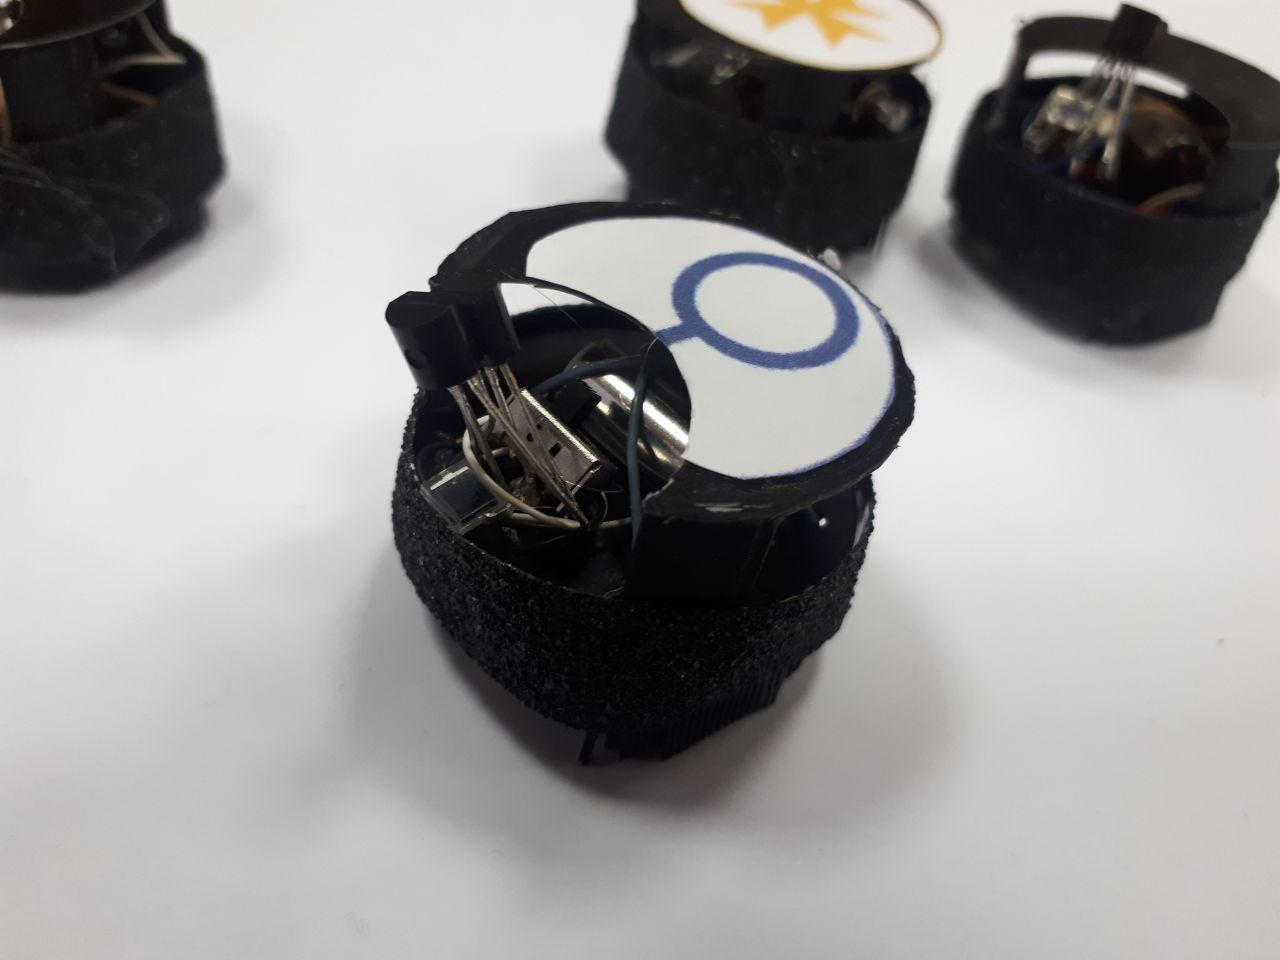
\includegraphics[width=\textwidth]{robot}
				\end{center}
			\end{column}
		\end{columns}
	\end{frame}

	\section{Результаты эксперимента}
	\begin{frame}
		\frametitle{\insertsection}
		
	\end{frame}
	
	
\end{document}